\documentclass[a4paper,11pt]{article}
\usepackage[margin=2cm]{geometry}		
\usepackage{uglix}
\usepackage{graphicx}
\pagestyle{plain}
\usepackage{array}
\newcommand{\tabstrut}{\vrule height 1.25em depth 0.5em width 0pt}

\begin{document}
\titre{CH08 - Feuille 02}{\textsc{BTSSIO}}{03/2020}
	
\exo{}

Pour chaque relation de E (en rose à gauche) vers F (en vert à droite) indiquer si c'est une application, et si elle est injective, surjective, bijective ou rien du tout. 

\begin{multicols}{2}

\def\myw{5cm}
\begin{enumerate}[\bfseries 1.]
	\item 	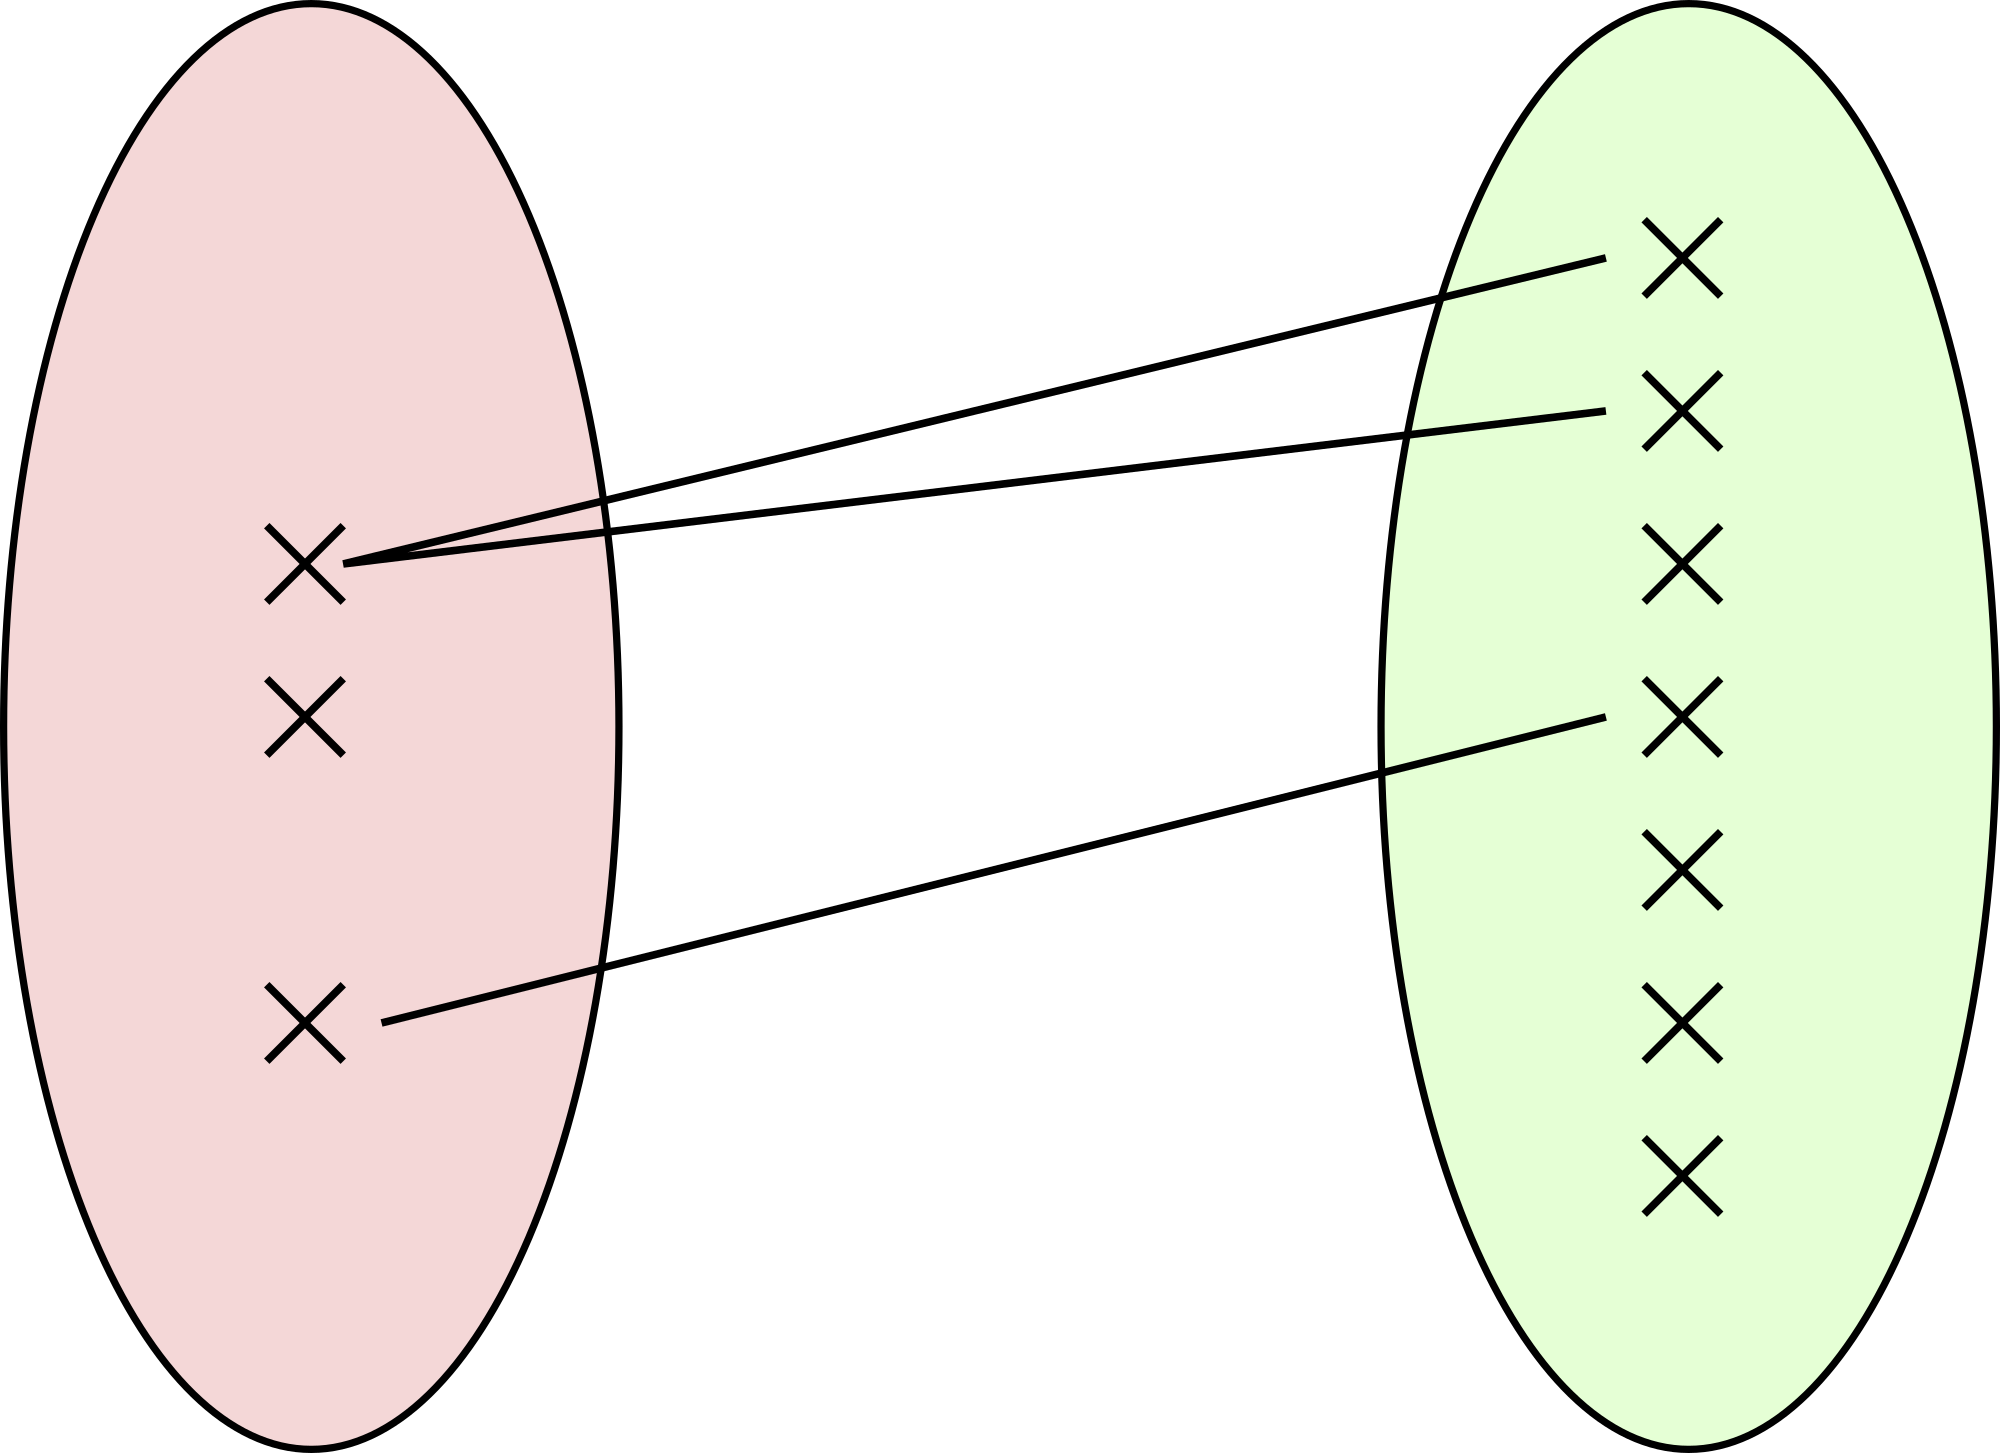
\includegraphics[width=\myw]{1.png}\\
	
			.\dotfill

	\item 	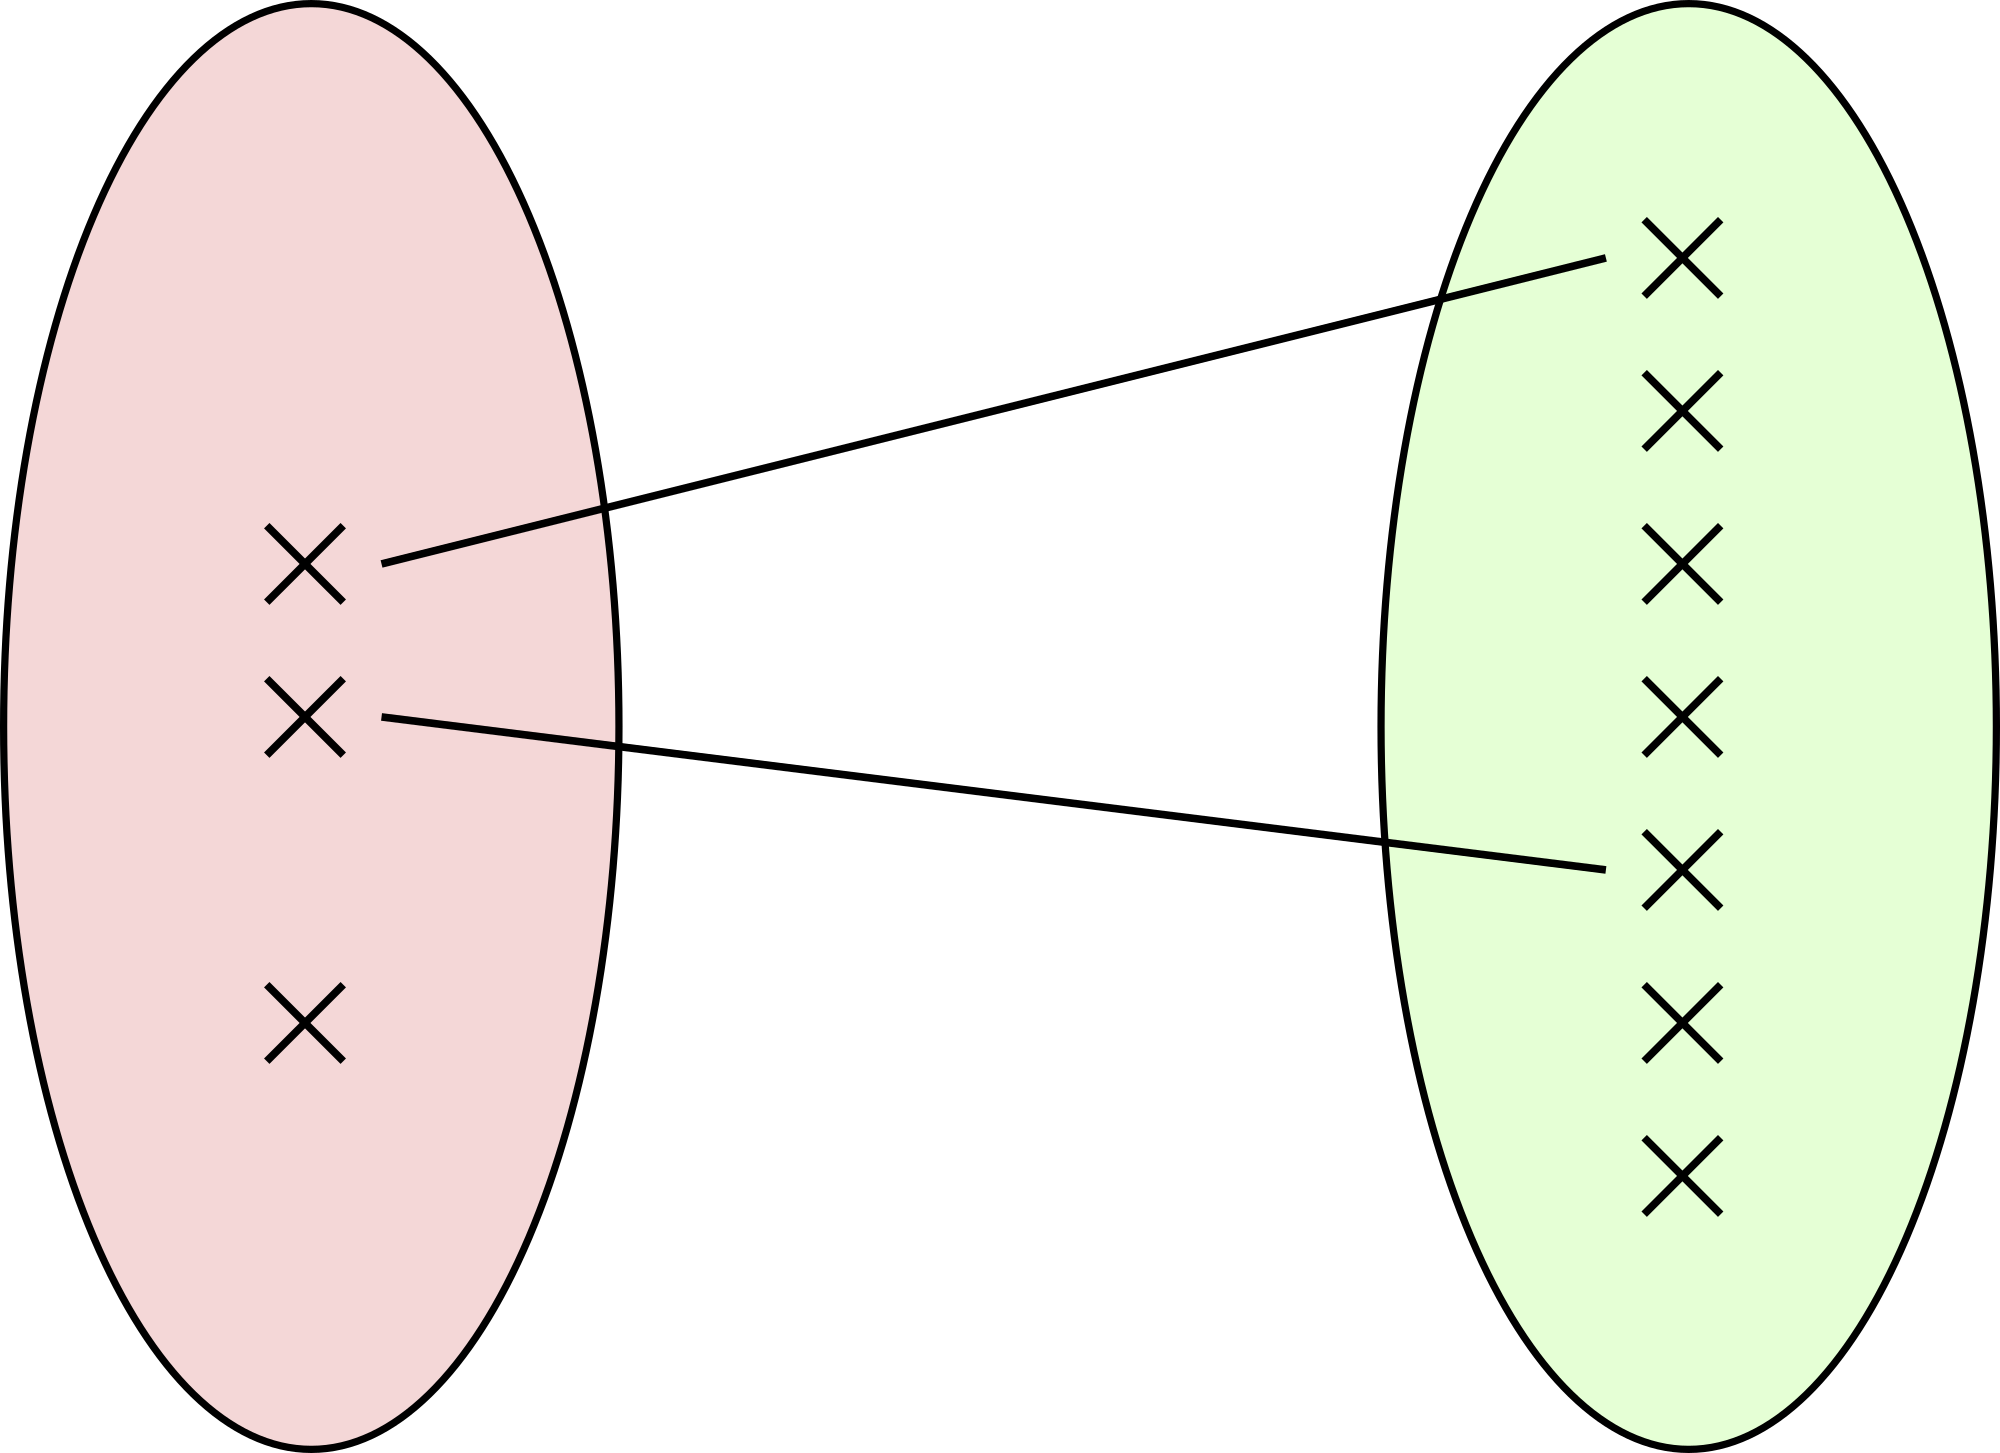
\includegraphics[width=\myw]{2.png}\\
	
			.\dotfill
	\item 	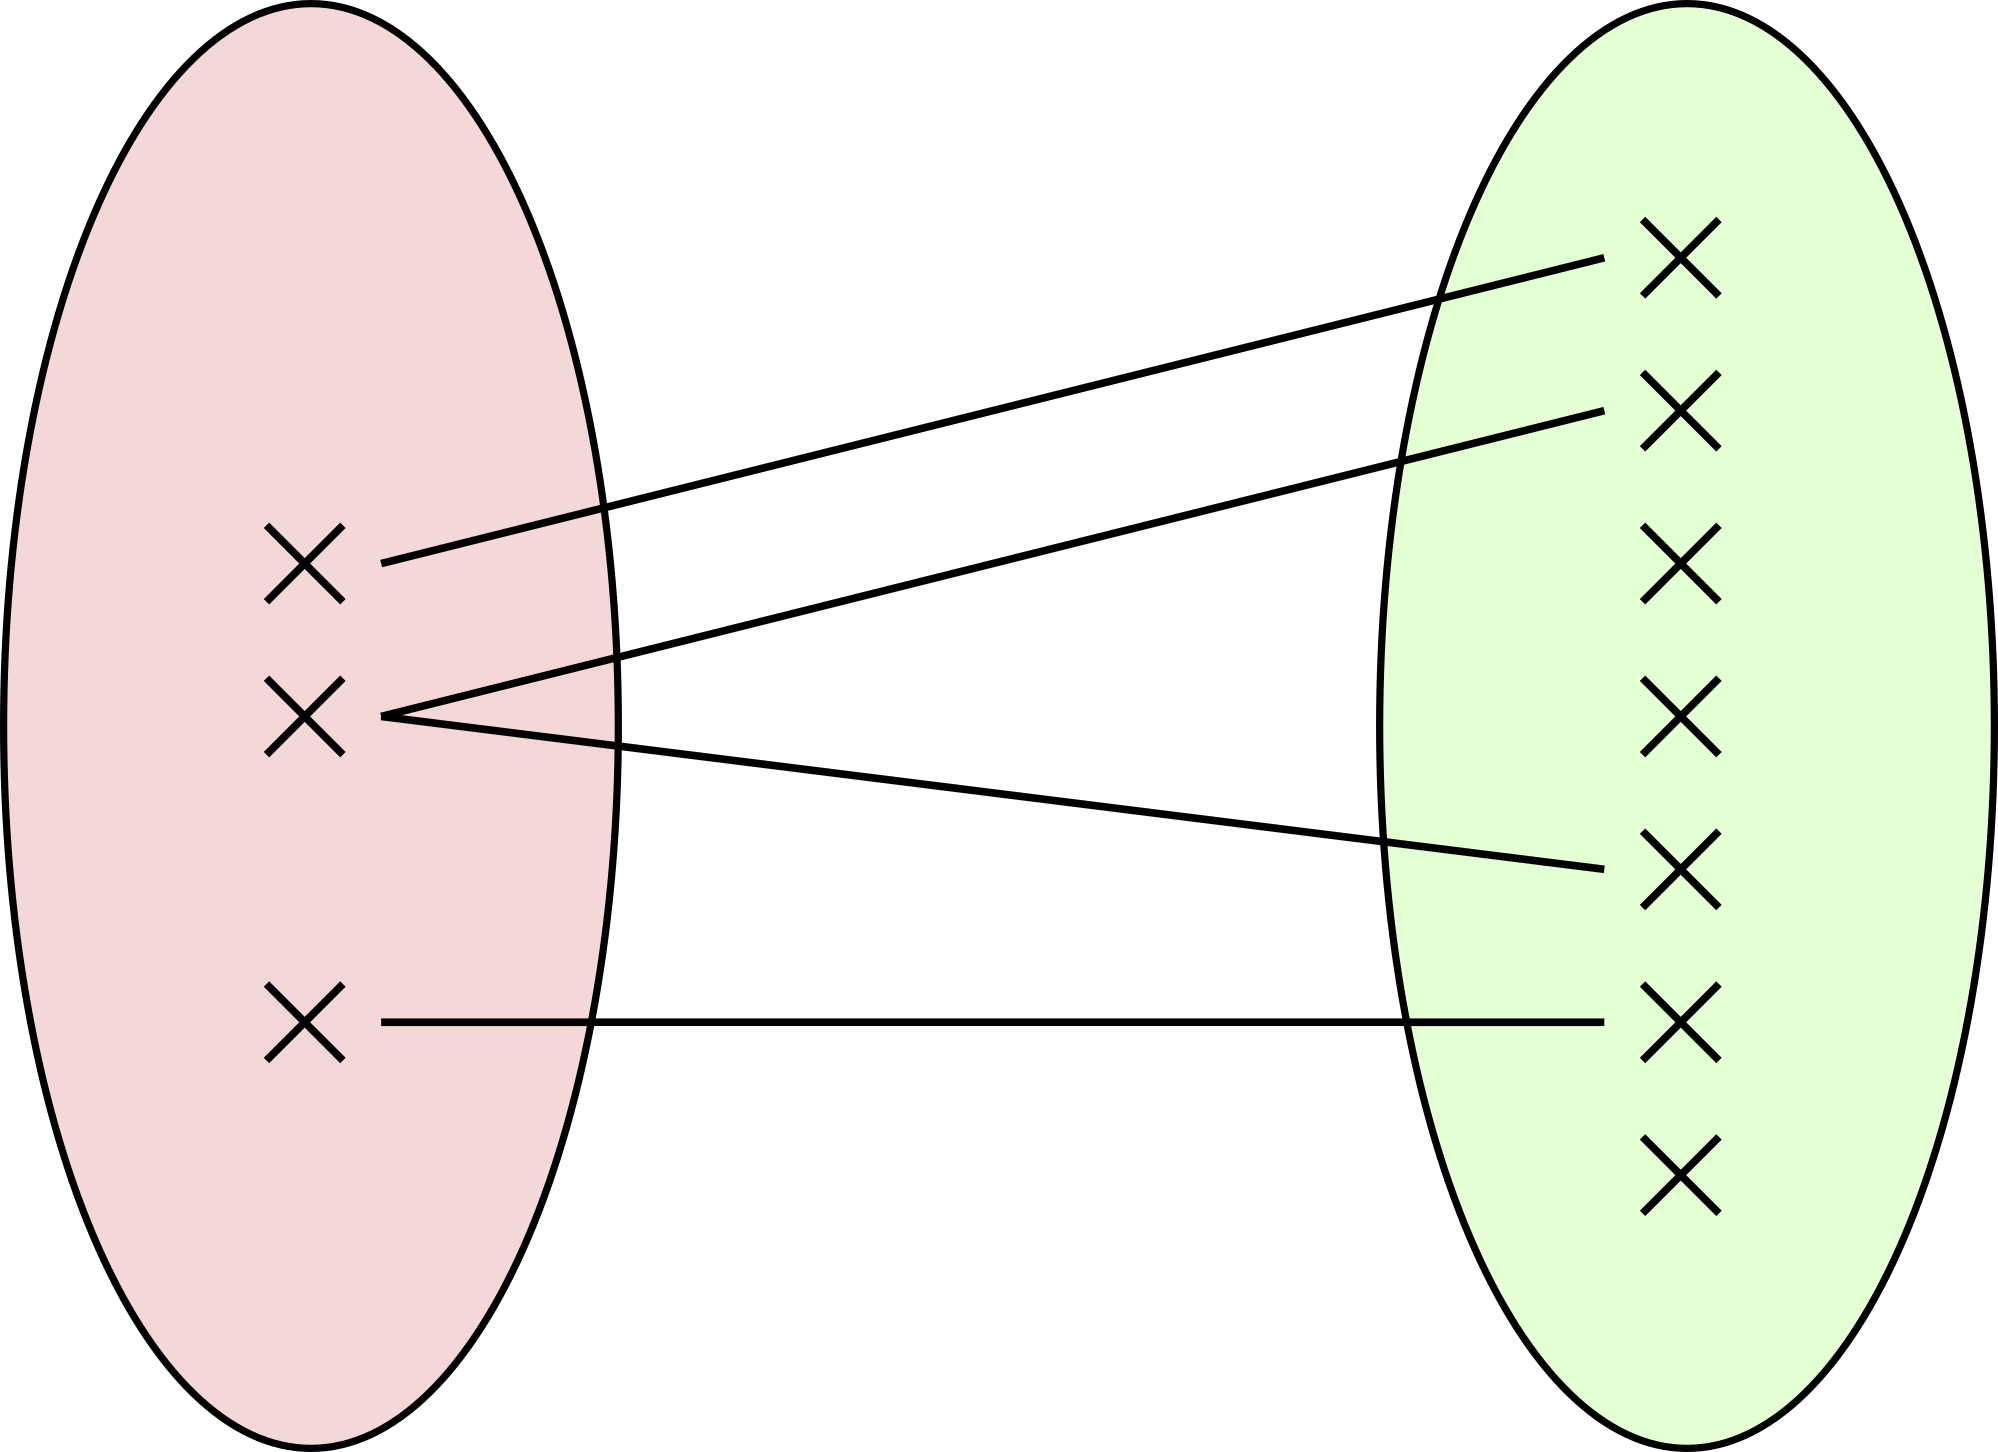
\includegraphics[width=\myw]{3.png}\\
	
			.\dotfill
	\item 	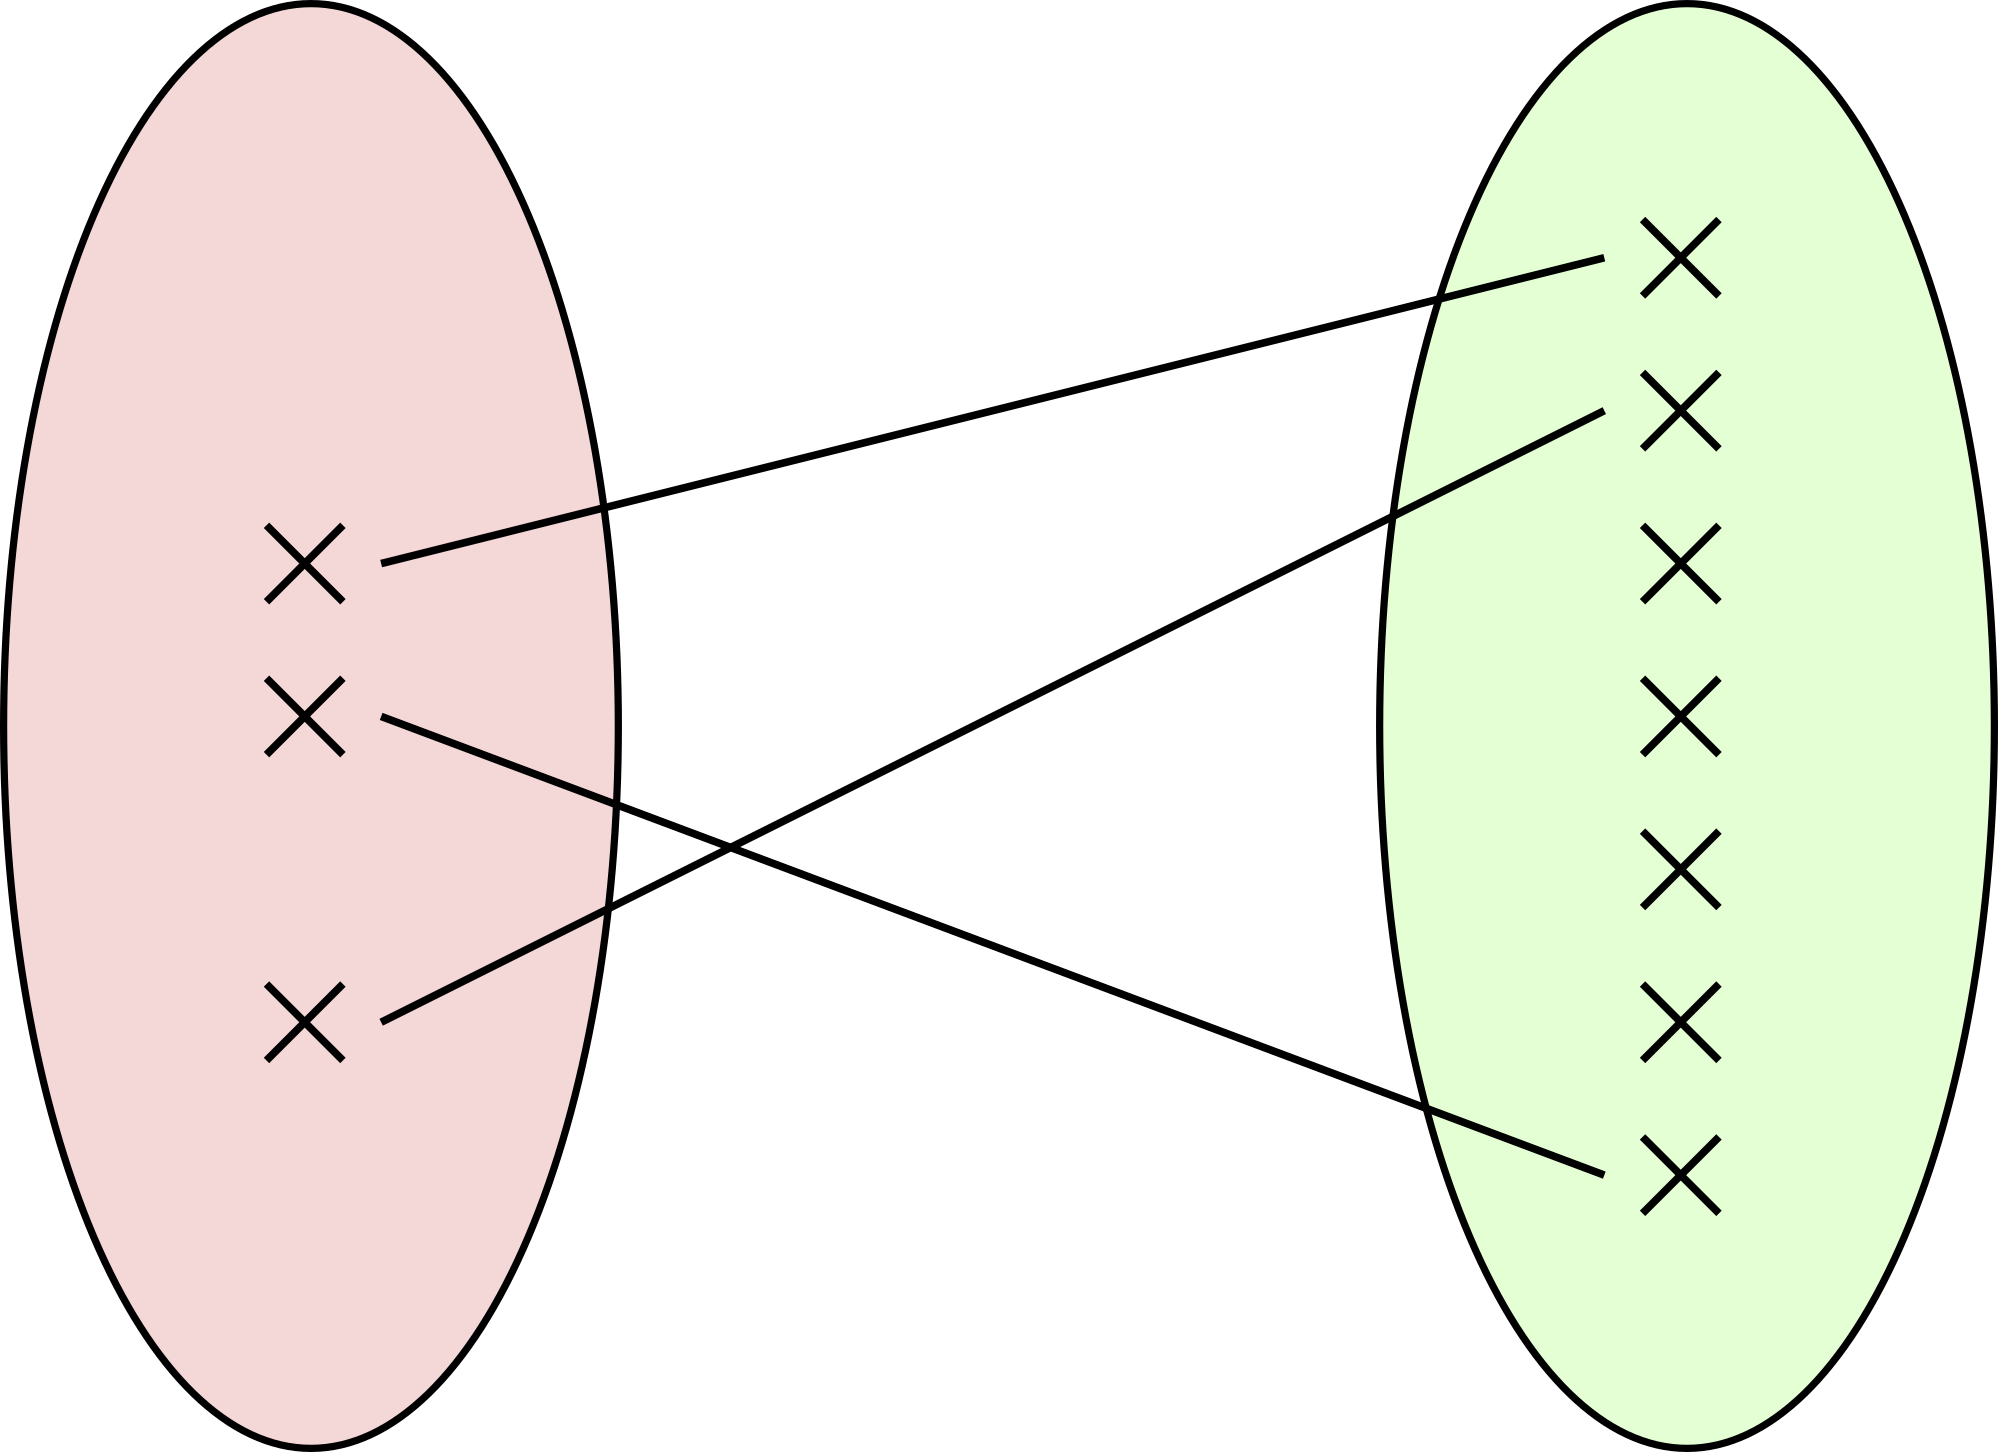
\includegraphics[width=\myw]{4.png}\\
	
				.\dotfill

	\item 	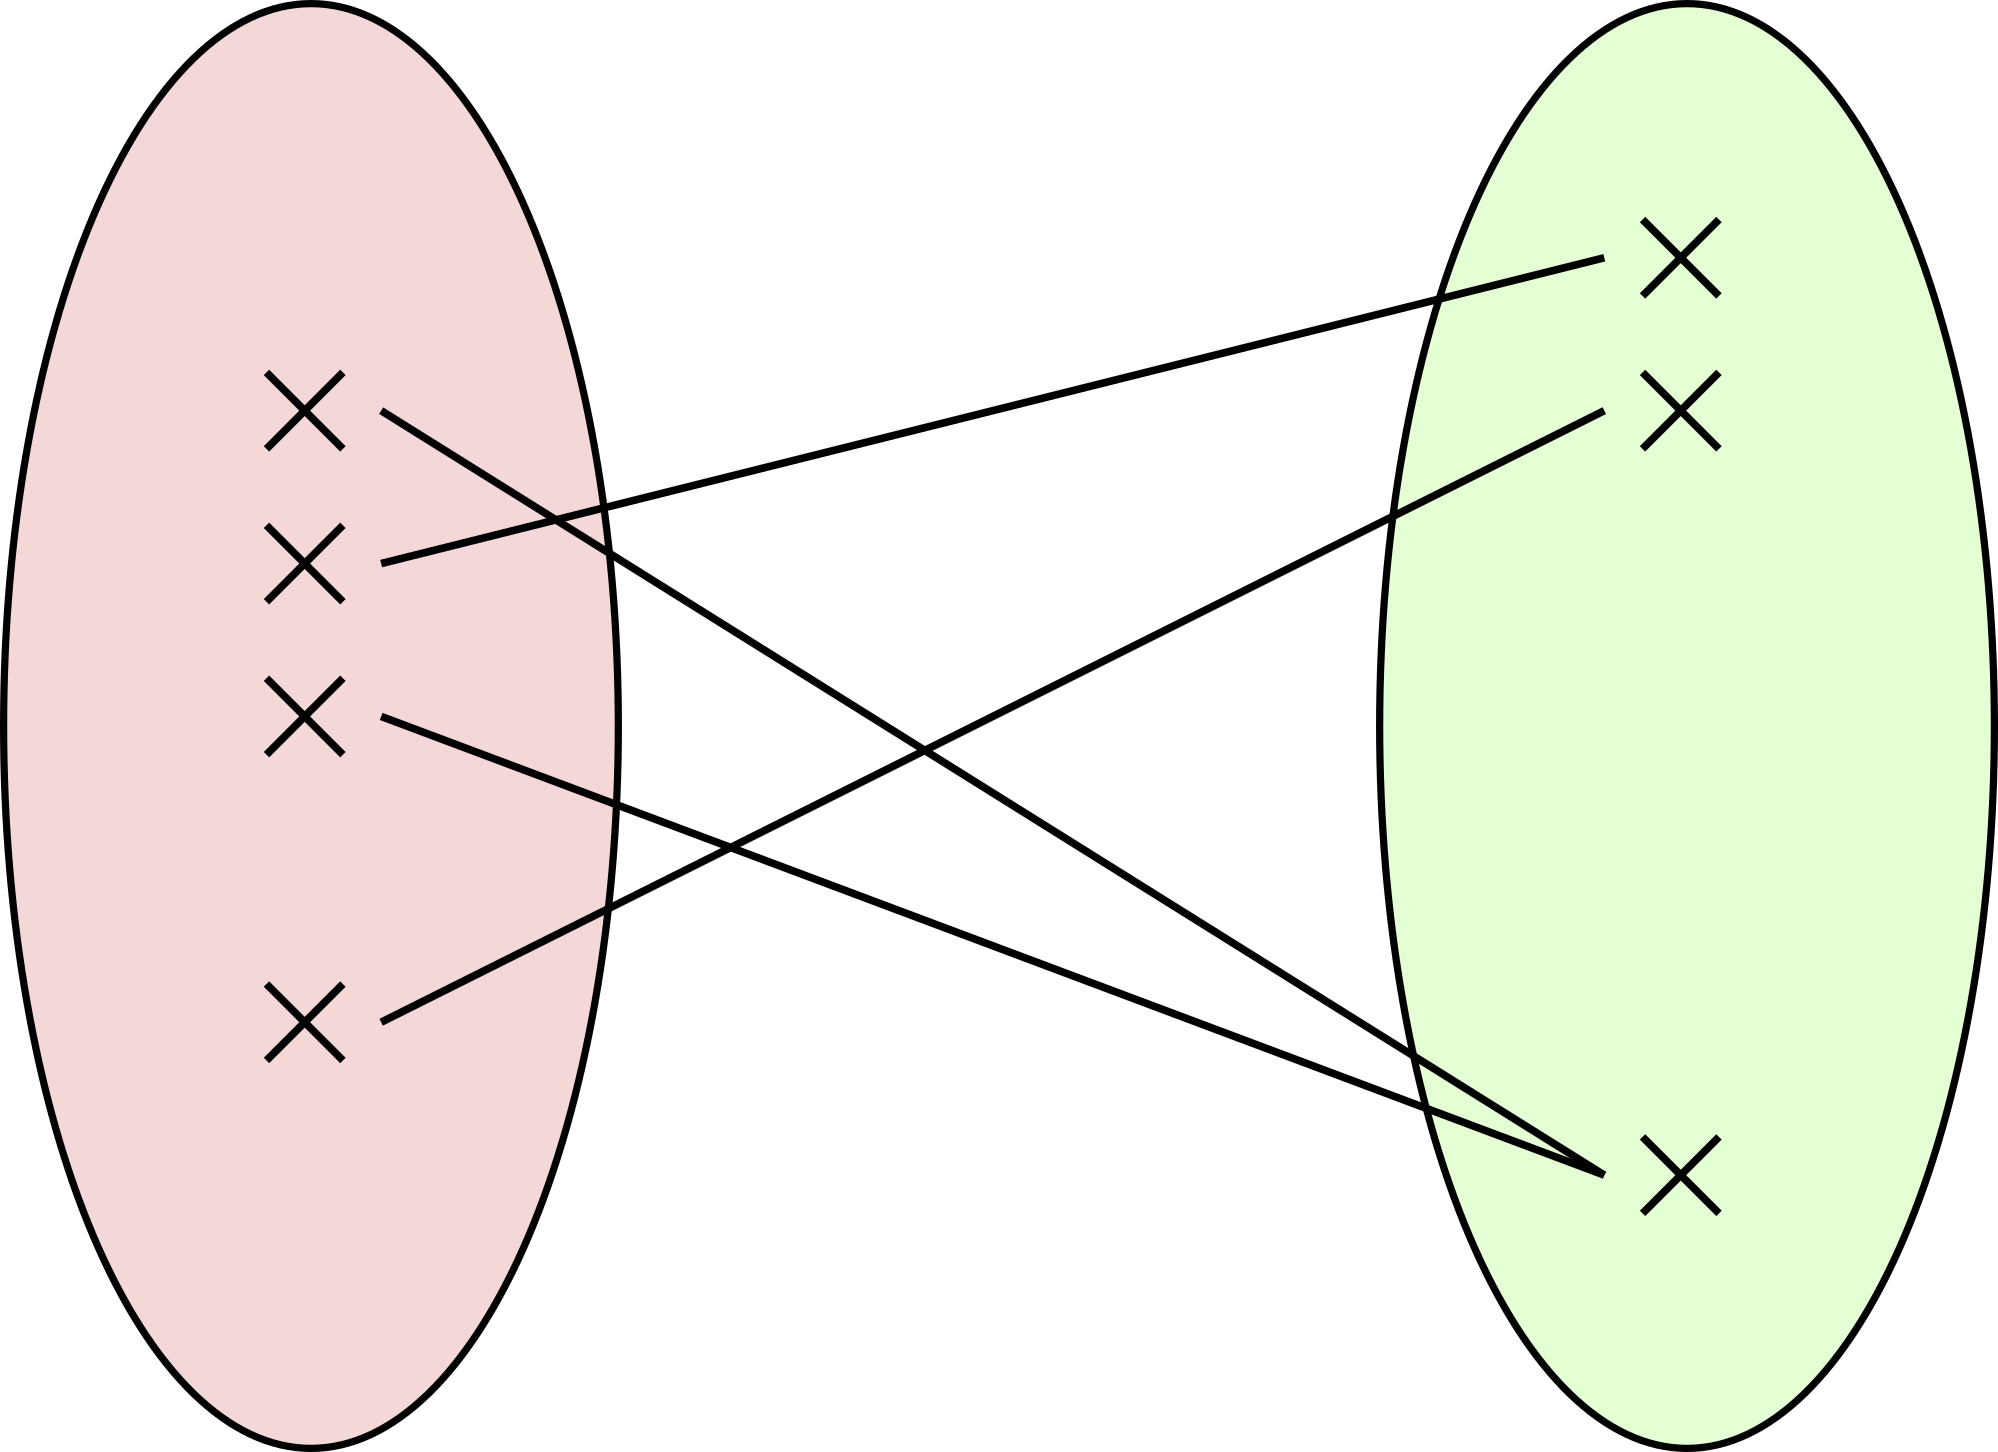
\includegraphics[width=\myw]{5.png}\\
	
				.\dotfill

	\item 	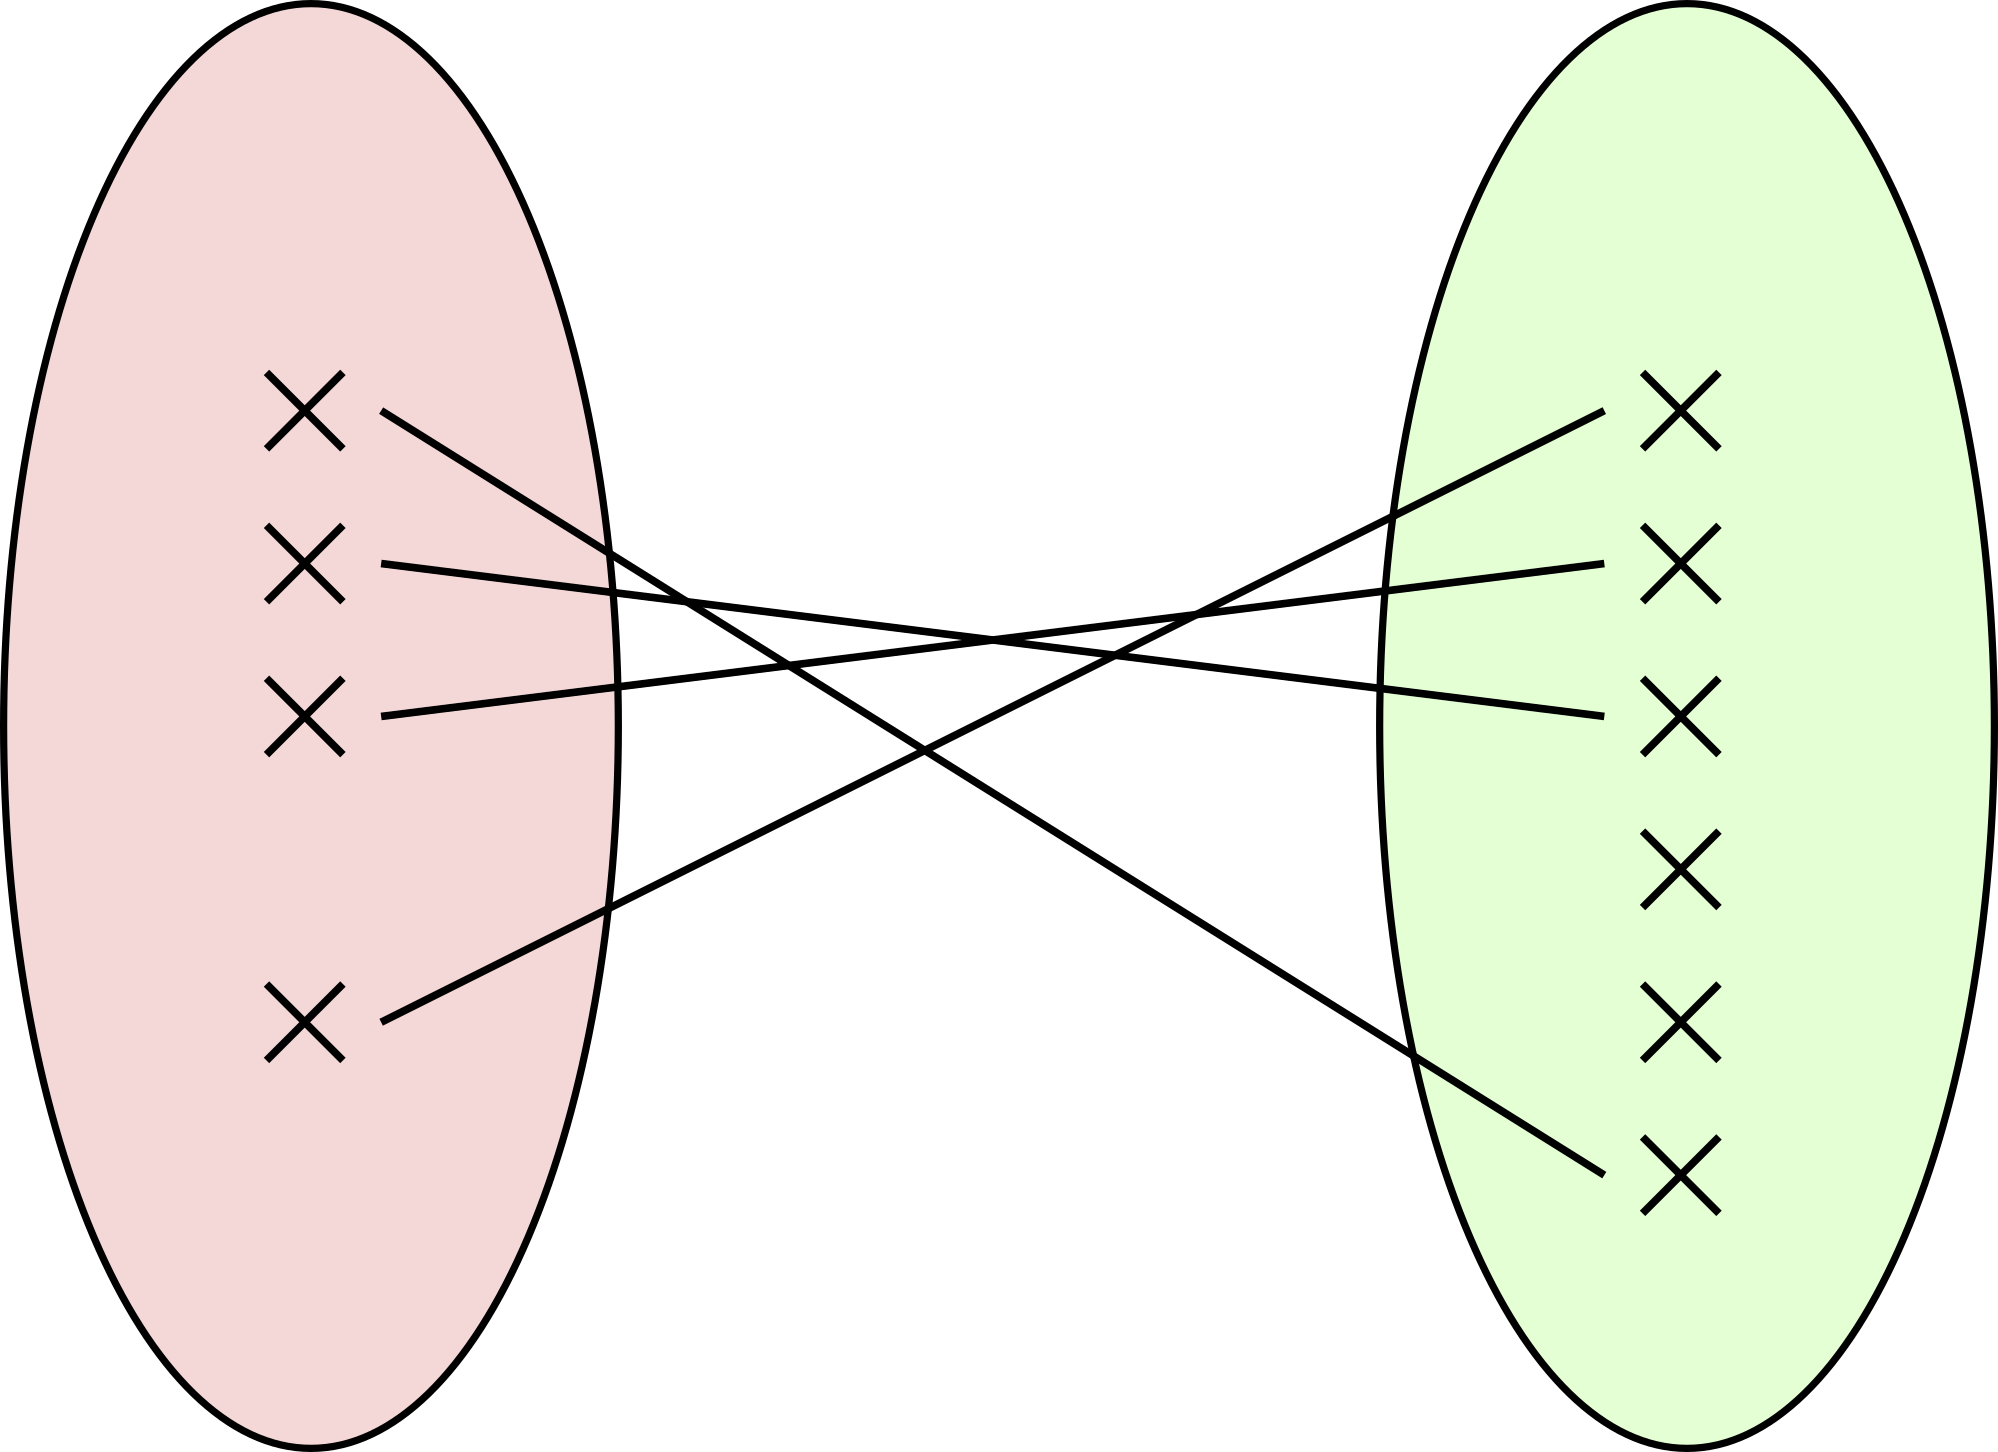
\includegraphics[width=\myw]{6.png}\\
	
				.\dotfill
	
	\item 	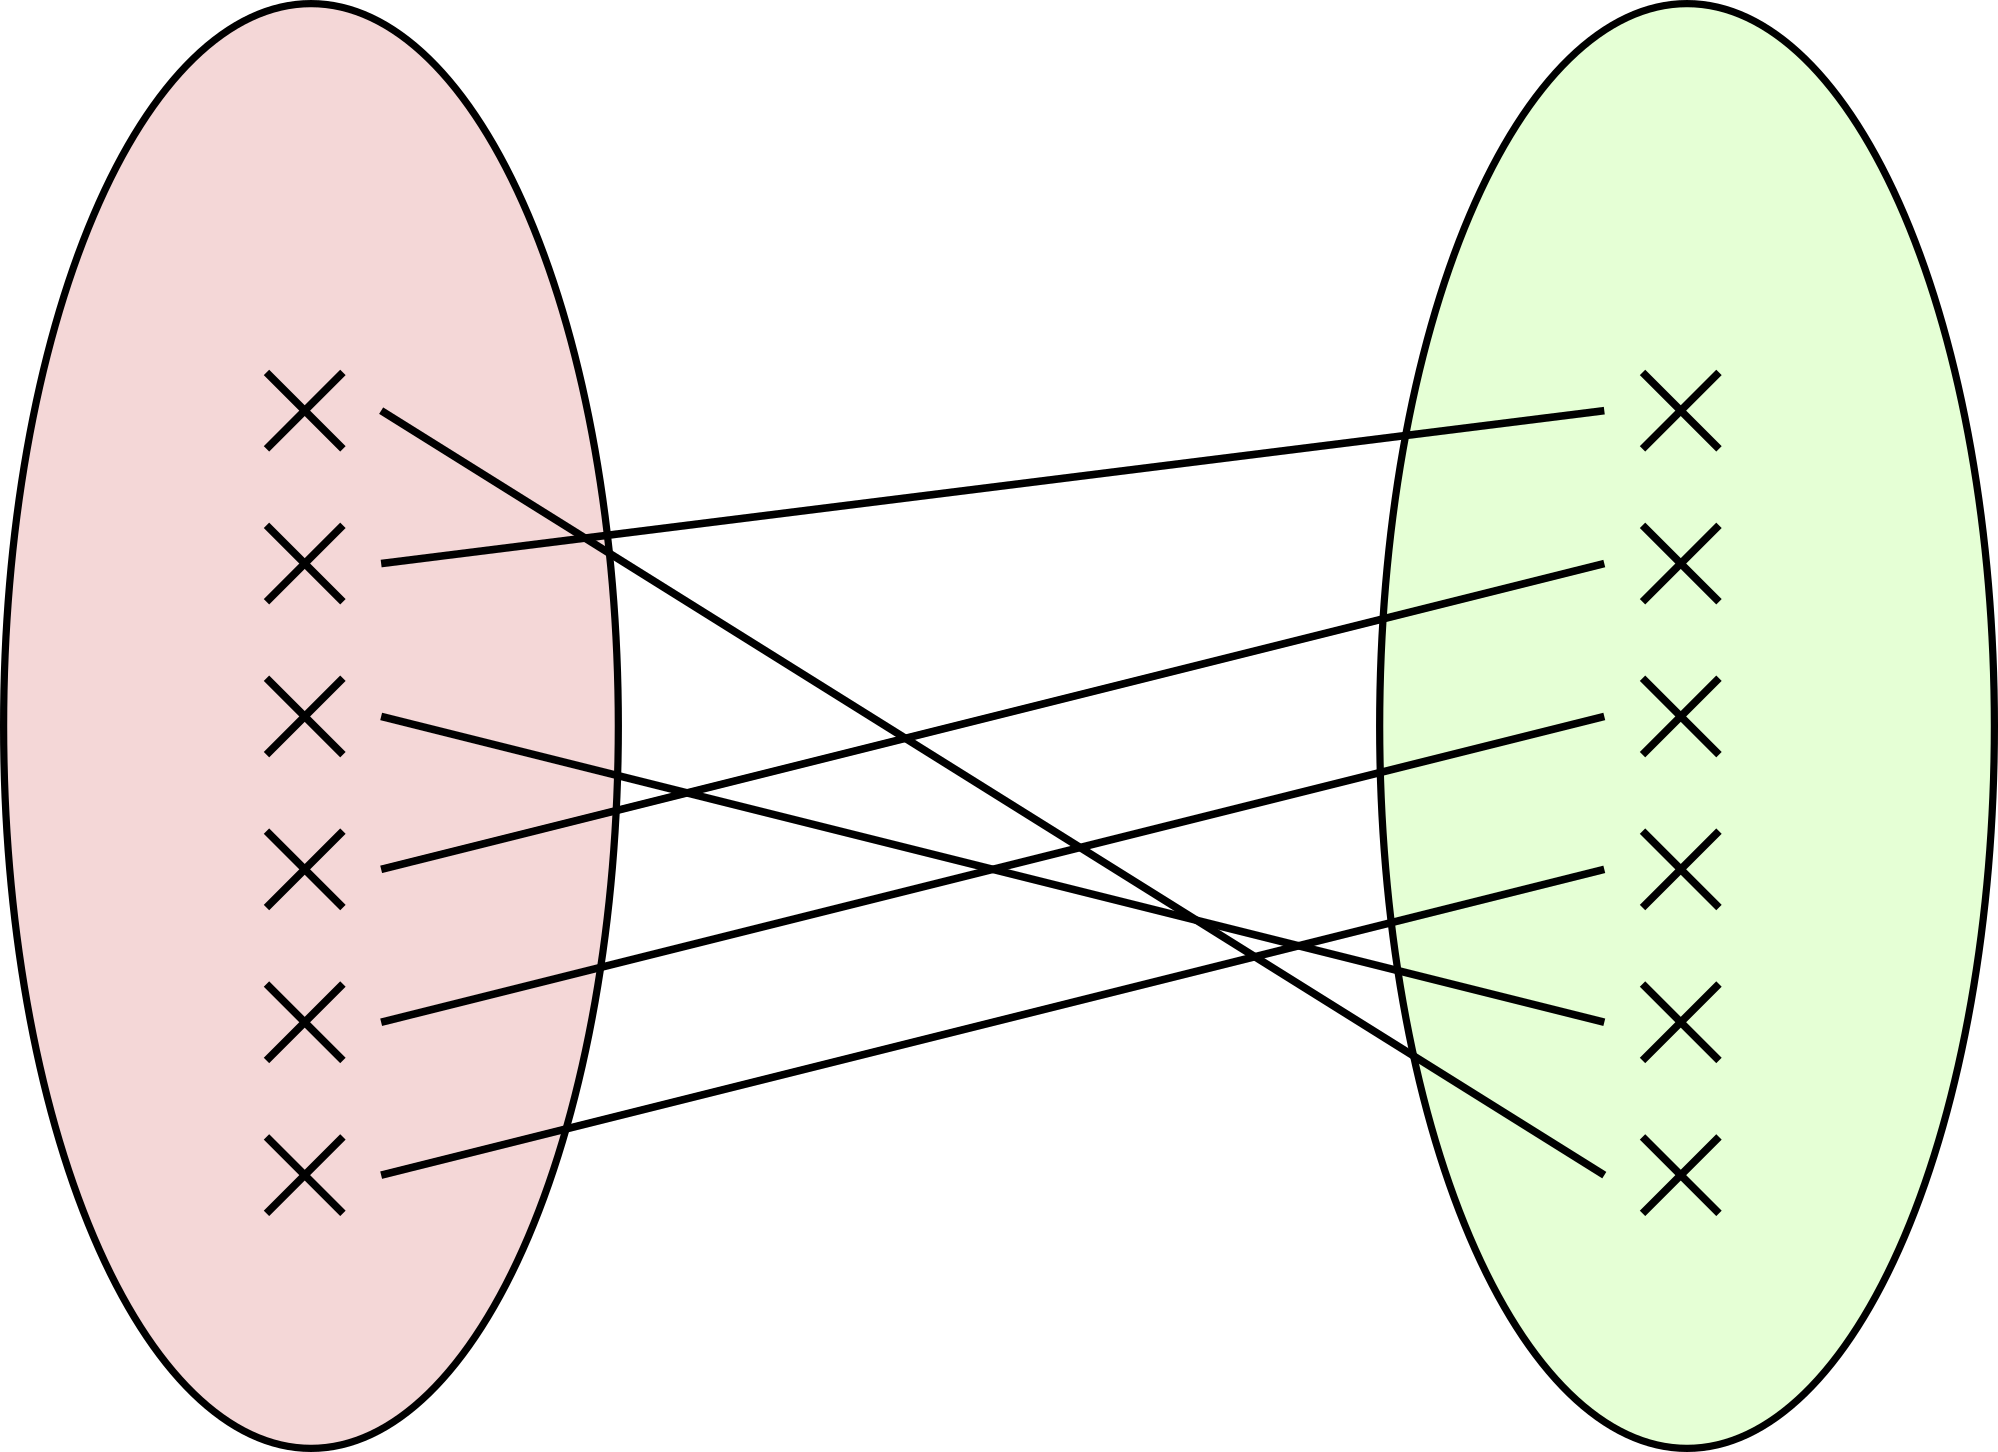
\includegraphics[width=\myw]{7.png}\\
	
				.\dotfill
		
		
	\item 	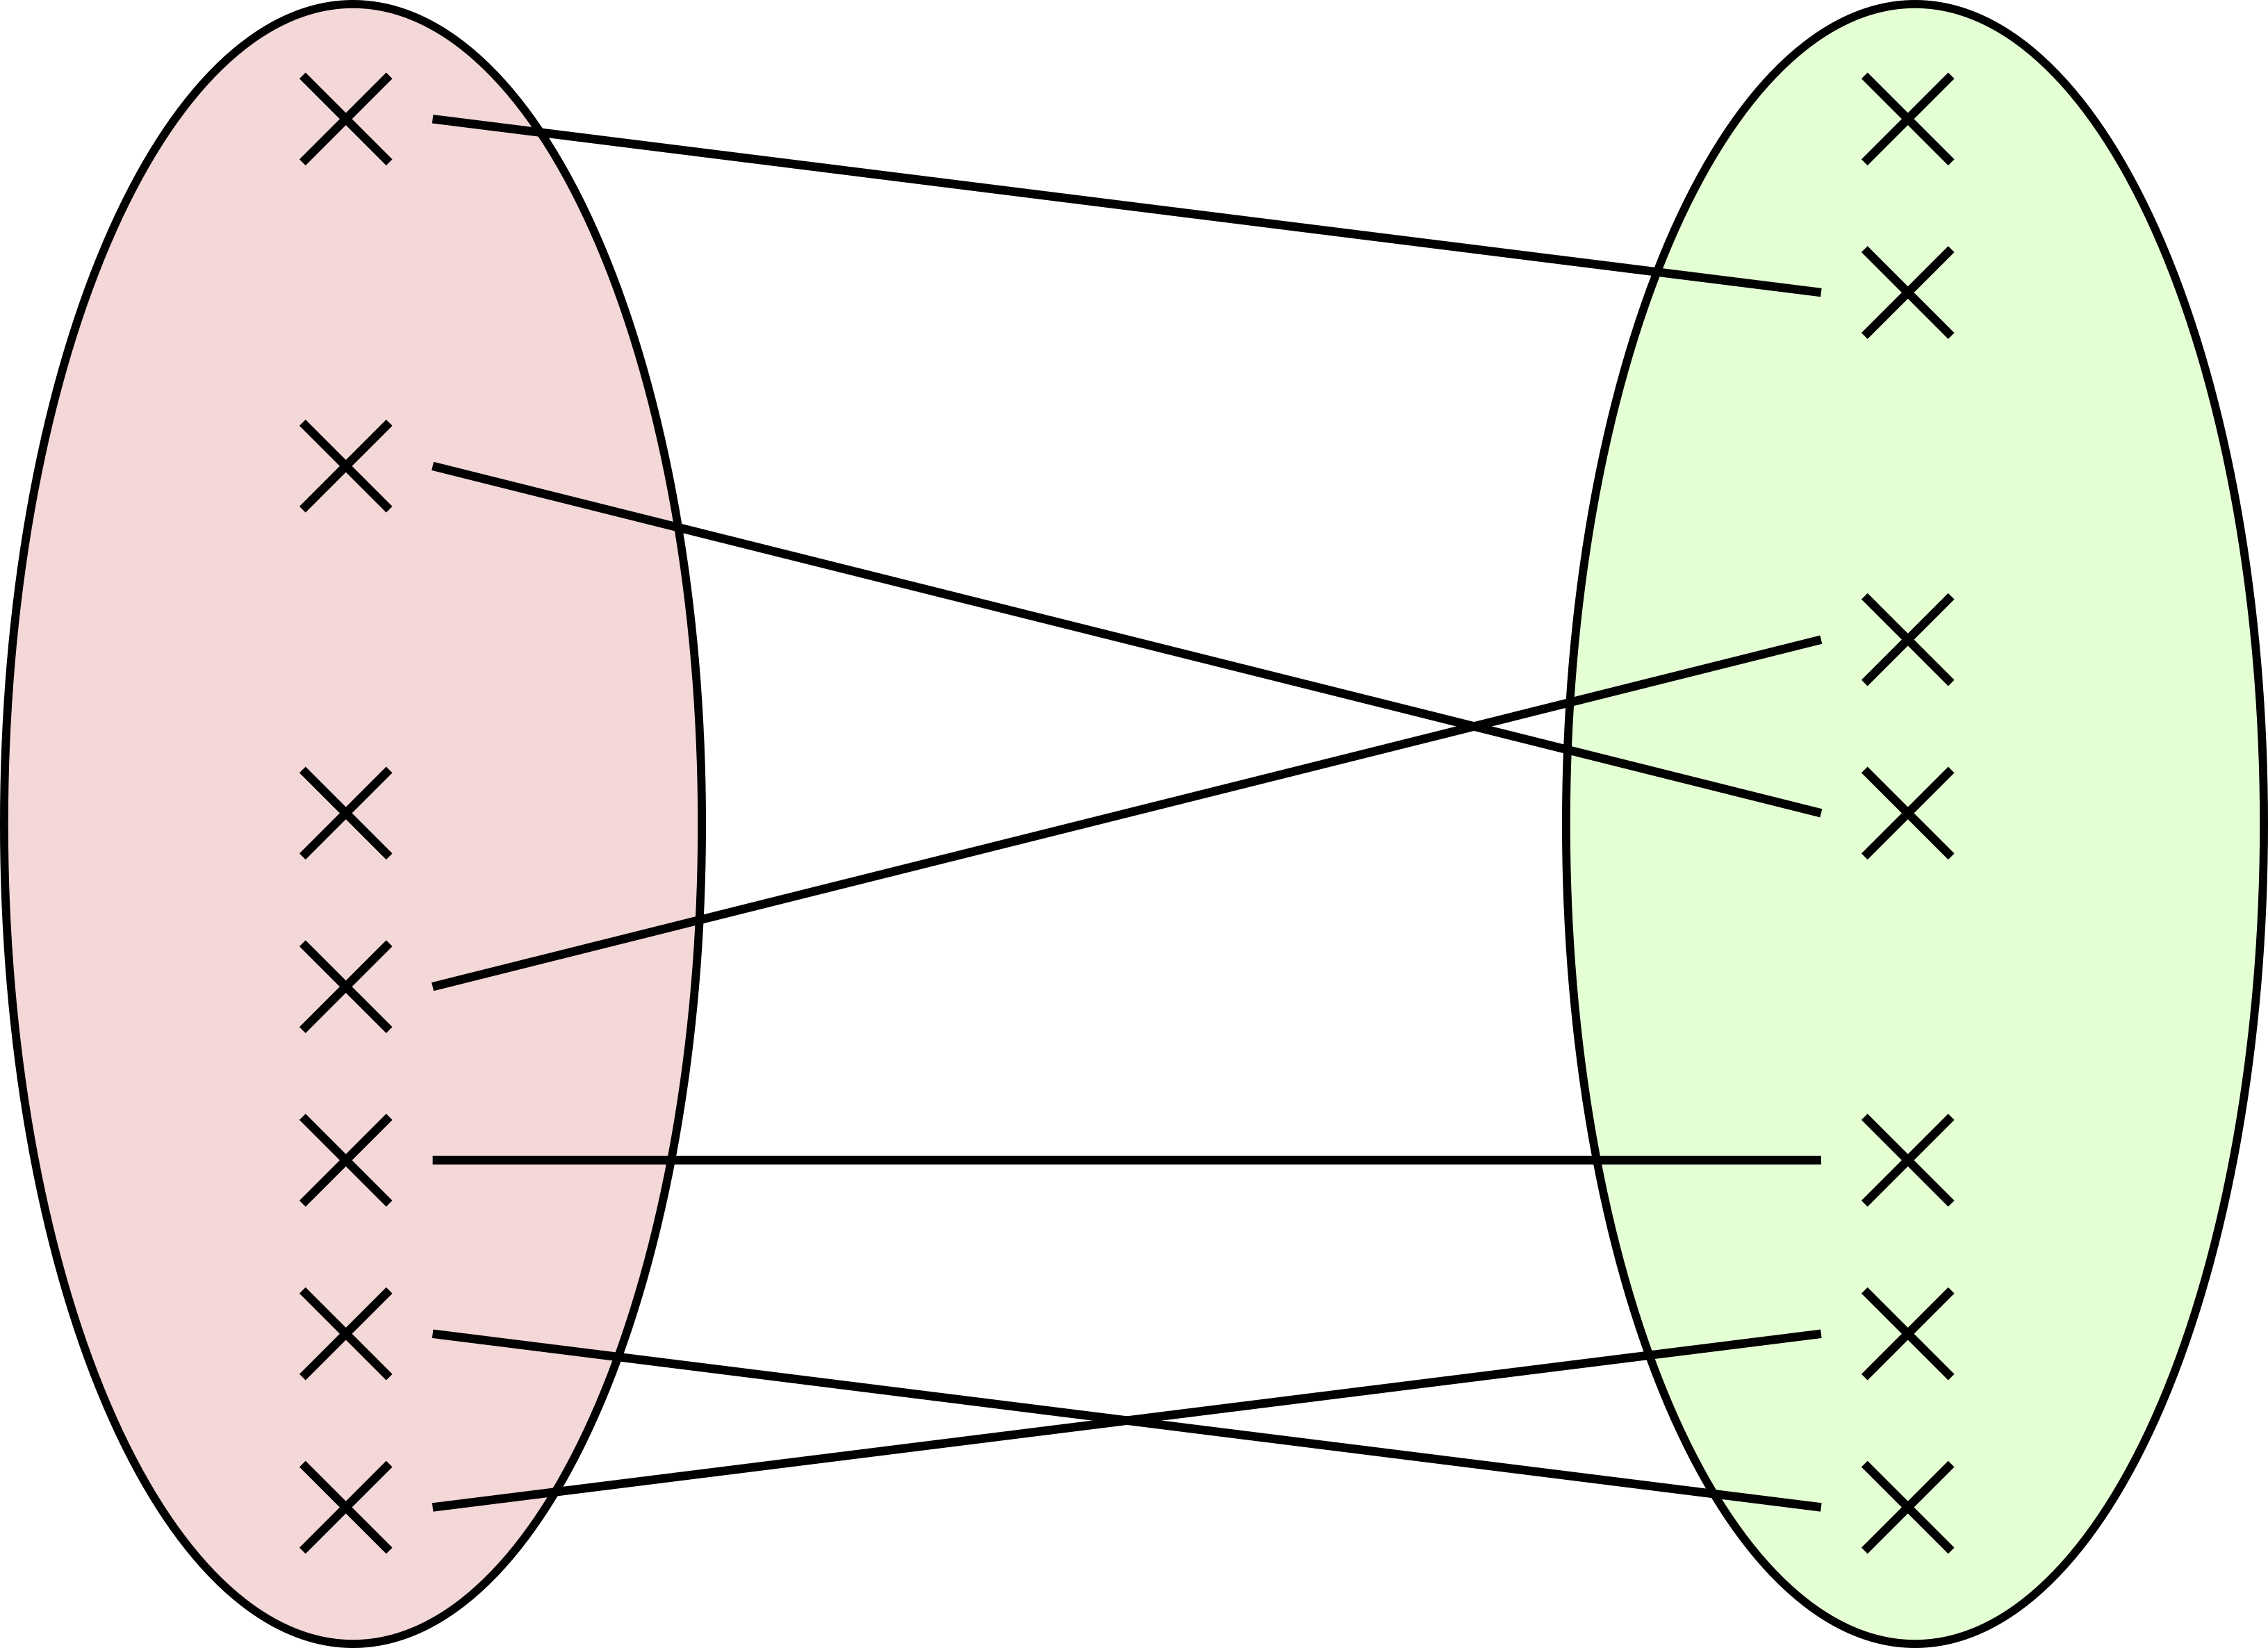
\includegraphics[width=\myw]{8.png}\\
	
				.\dotfill
\end{enumerate}
\end{multicols}

\exo{}


$E=\{0;1;2;3;4;5;6;7\}$ et $F=\{0;1;2;3\}$.\\
$f$ est l'application de $E$ dans $F$ qui à tout élément de $E$ associe son reste dans la division euclidienne par 3.
\begin{enumerate}[\bfseries 1.]
	\item 	$f$ est-elle injective ? Surjective ?
	\item 	Posons $A=\{1;3;4\}$, déterminer $f(A)$, puis posant $B=f(A)$, déterminer $f^{-1}(B)$.
	\item 	Posons $C=\{2;3\}$, déterminer $f^{-1}(C)$, puis, en posant $D=f^{-1}(C)$, déterminer $f(D)$.\\
\end{enumerate}

\exo{}

Soit $f$ l'application de $\R$. dans $\R$. définie par $f(x) = 4x + 10$.
\begin{enumerate}[\bfseries 1.]
	\item 	f est-elle une injection ?
	\item 	f est-elle une surjection ?
	\item 	f est-elle une bijection ?
	\item 	Déterminer l'image directe de $\fif{2}{3}$ et de $\fii{0}$.
	\item 	Déterminer l'image réciproque de $\fii{0}$.\\	
\end{enumerate}

\exo{}

$E=\{a;b;c;d\}$, $F=\{1;2;3\}$ et $G\{\alpha;\beta;\gamma\}$.\\
$f$ est définie de $E$ dans $F$  et $g$ de $F$ dans $G$ par\\
$f(a)=2$, $f(b)=1$, $f(c)=3$ et $g(1)=\gamma$, $g(2)=\alpha$ et $g(3)=\beta$.

\begin{enumerate}[\bfseries 1.]
	\item 	$f$ et $g$ sont-elles injectives ? Surjectives ? Bijectives ?
	\item 	Définir l'application $g\, o\, f$.
	\item 	Peut-on définir l'application réciproque de $f$ ? De $g$ ?
\end{enumerate}

\exo{*}

Expliciter  $f\,o\, g$ et $g\,o\, f$ lorsque $f$ et $g$ 
sont les fonctions suivantes :
\begin{multicols}{2}
\begin{tabbing}
$f\ :\ $	\=	$\R$	\=	$\longrightarrow$	\=	$\R$\\
		\>	$x$		\> 	$\longmapsto$		\>	$x^2+2$
\end{tabbing}
\begin{tabbing}
$g\ :\ $	\=	$\oii{0}$	\=	$\longrightarrow$	\=	$\R$\\
			\>	$x$		\> 	$\longmapsto$		\>	$\dfrac{1}{\sqrt{x}-1}$
\end{tabbing}
\end{multicols}
\end{document}
